\section{Data sets}
\label{sec:observations}


\begin{figure*}

    \centering
    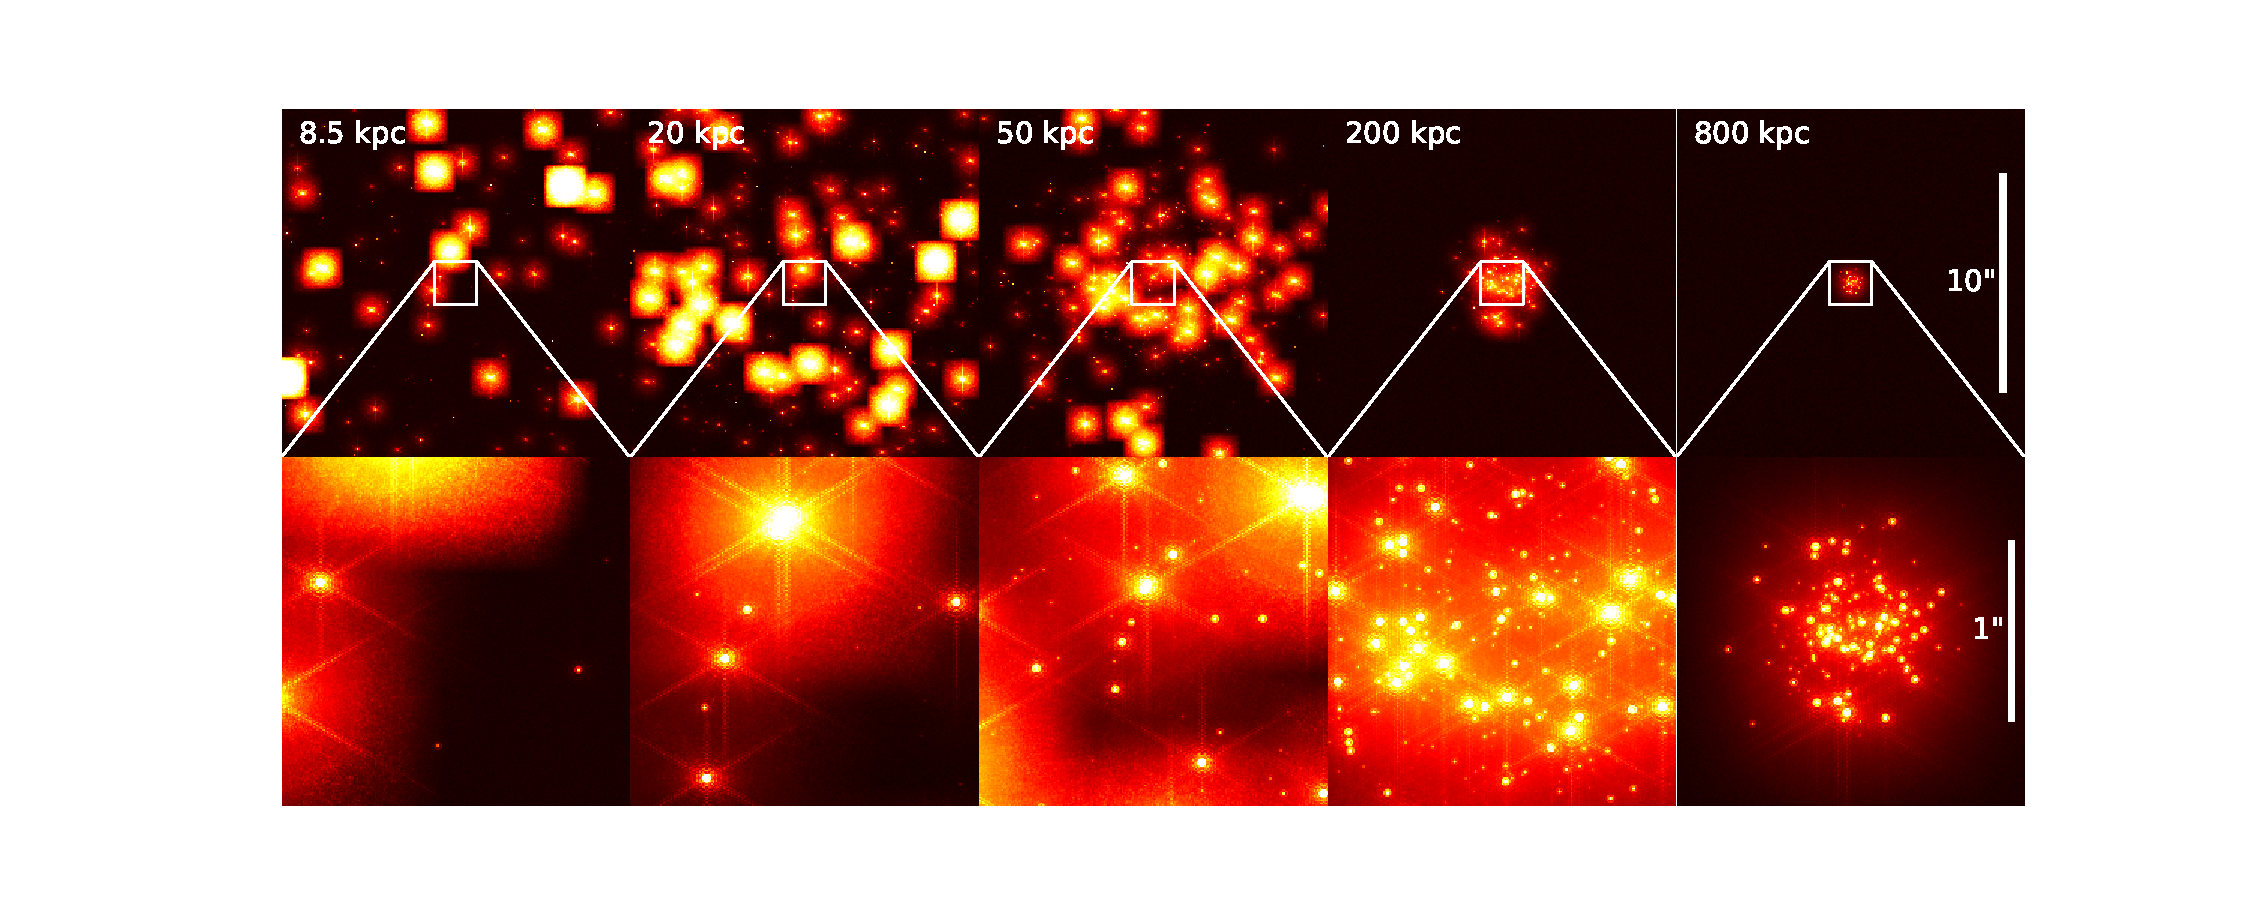
\includegraphics[width=\textwidth]{images/5_clusters.pdf}

    \caption{An illustration of the data set we used for this study. The young massive cluster depicted here contains a mass of 2$\times$10$^4$\,\msun and has a half-light radius of 1\,pc. It was observed with the MICADO instrument simulator at distances from 8\,kpc to 800\,kpc. The top row shows the cluster as seen by the centre detector of MICADO. The bottom row shows a 2``$\times$2`` window (512$\times$512 pixels) at the centre of this detector, corresponding to the area we used for our study. \rewrite ASK MAORY ABOUT NEW PSF - REDO WITH CLENET PSF
    }
    
    \label{fig:5_clusters}
    
\end{figure*}


\begin{figure*}

    \centering
    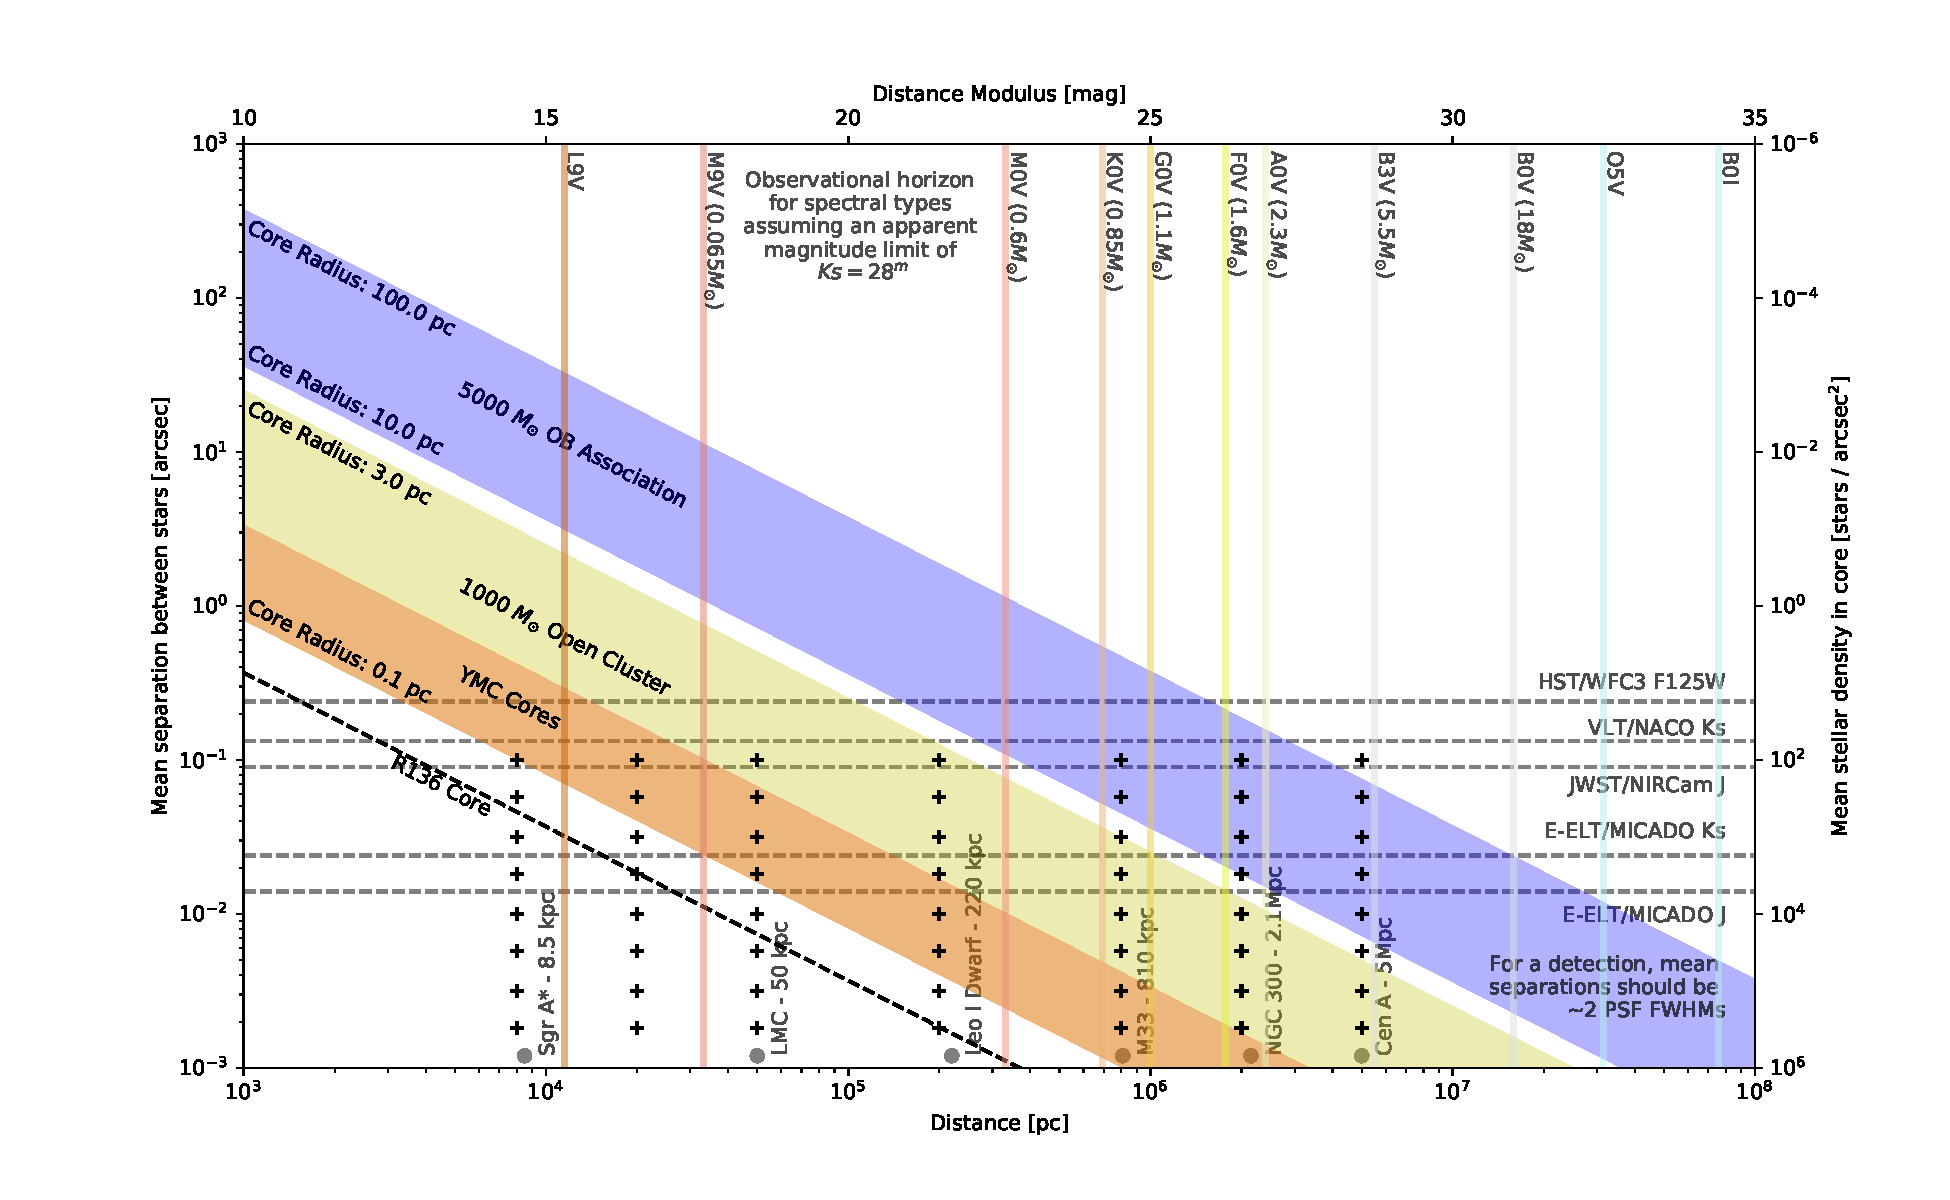
\includegraphics[width=\textwidth]{images/resolved_stellar_densities.pdf}

    \caption{The on-sky stellar density parameter space covered by the dense stellar fields in this study (crosses). 
    The diagonal bands show the range of core stellar densities for the three major categories of young stellar populations: young massive clusters (orange), open clusters (green), and OB associations (blue). 
    The vertical lines represent the furthest distance at which a certain type of main sequence star will still be above the detection limit of MICADO, i.e. Ks=28\m.
    The dashed horizontal lines show the theoretical confusion limit for MICADO/ELT, JWST, HST and an instrument similar to NACO/VLT. The confusion limit assumes an average minimum distance of 2$\times$ the PSF FWHM between stars.
    \rewrite REMOVE excess crossed
    }
    
    \label{fig:resolved_stellar_densities}
    
\end{figure*}


The most reliable way to determine the IMF is to look at a population of stars which is still young enough for all the original members to still be around, yet old enough that the main phase of star formation activity has ceased. 
If a population is too young, it will not have finished forming all its stars and dust extinction will be a major source of uncertainty and incompleteness. Too old and the most massive members will already have exploded as supernovae. 
Dynamical effects will also have lead to evaporation of stars from the cluster, posing a problem to IMF completeness.
Unfortunately such ideal conditions are rarely observed. 
Star formation happens on time scales of 10\h6 years. 
The most massive stars burn their hydrogen reserves within the first several ten million years and move off the main sequence\needcite. 
Given that the dispersion time for stellar clusters is on the order of hundreds of millions of years, at any point in time relatively few of the observable new clusters will be found in the ideal age range (between 5 and 20\,Myr) for studying the IMF\needcite. 
The majority of IMF studies focus on the clusters which come closest to meeting these conditions - namely the cores of open clusters (OC) and young massive clusters (YMC)\needcite. 
It should be mentioned that OB associations also provide a laboratory for studying the IMF. 
However as these are older and in many cases more spread out, the chances of contamination from background sources and missing ejected stars is higher\needcite. 
% Furthermore, the high mass end of the IMF cannot be reliably observed as the highest mass stars have already left the main sequence, and some have ended as supernova\correct.


\subsection{Parameter Space}

HST has a diffraction limit of \s0.1'' at 1.2\,\um and can reach magnitudes as faint as J=28.6\m \citep{hst_wfc3} in a 10 hour observation. Using AO assisted ground based instruments similar to NACO at the VLT, diffraction limited observations can be achieved over small (\s1') fields of view. 
The diffraction limit of the VLT telescopes (\s0.03'' at 1.2\,\um) is 3$\times$ smaller than HST, however due to the atmospheric background the sensitivity limits of VLT instruments are many magnitudes brighter than for HST. 
As boundary conditions for our suite of stellar fields we took the resolution limit of HST, as cluster cores with densities lower than this are already accessible to the HST. 
Assuming an average of one star per FWHM of the PSF, our lower density limit was set to 100\,\spa. 
For the upper density limit we first took the theoretical diffraction limit of the ELT: 7\,mas at 1.2\,\ume, or 2$\times$10\h4\,\spae. However as faint stars drop below the telescope's detection limit the effective density of detectable stars decreases with increasing distance. 
As we wanted crowding limited observations at large distances (\textgreater1\,Mpc), we increased the true stellar density by a factor of 15$\times$ so that the M\,\textgreater\,1\,\msun stars alone would meet the crowding criterion of 1 star per FWHM. 
Thus we set the upper limit for the true cluster stellar density to 3$\times$10\h5\,\spa.

Current telescopes are capable of detecting almost all main sequence stars above the hydrogen burning limit (\s0.08\,\msune) within a few kiloparsecs of the Sun\needcite. 
Detecting all main sequence stars in clusters further afield, e.g. in the galactic centre and beyond, is where MICADO's increased sensitivity and resolution will bring the greatest breakthroughs. 
Indeed the question of whether the IMF is truly universal dictates that we study the IMF outside the Milky Way. 
Therefore we placed our model proxy-clusters at distances corresponding to some of the more well known celestial landmarks: The Galactic Centre (\s8\,kpc), the LMC (\s50\,kpc), Leo I dwarf galaxy (\s200\,kpc), M33 (\s800\,kpc)\footnote{The author recognises that the location of the ELT in the southern hemisphere is unfavourable for effectively observing M33. We provide this data point because M33 will, with luck, be visible to the Thirty Meter Telescope.}, NGC 300 (\s2\,Mpc), and Cen A (\s5\,Mpc). 
Figure \ref{fig:resolved_stellar_densities} shows the parameter space covered by open clusters of average mass (\s1000\,\msun) with radii between 0.1\,pc and 3\,pc and OB Associations of average mass (\s5000\,\msun) with radii between 10\,pc and 100\,pc as distance from Earth increases. 
The lower bounds of the open cluster parameter space also covers the cores of YMCs. Average cluster properties were derived for the OB Associations from \citet{melnik1995}, for the open clusters from \citet{piskunov2007}, and for the YMCs from \citet{portegies2010}.



\subsection{Artificial stellar fields}

In this study we generated densely populated stellar fields, that could function as proxies for the dense regions at the cores of young stellar clusters. 
The parameter space covered by these cluster proxies are shown with the crosses in Figure \ref{fig:resolved_stellar_densities}. 
The size of each stellar field was set at 2''$\times$2'' (see section \ref{sec:telescope}). 
The stellar fields were populated by continually drawing stars from an IMF until the required stellar density was reached. 
The mass of each star was drawn at random from an IMF distribution with minimum and maximum masses of 0.01\,\msun and 300\,\msun. 
The IMF followed a standard \citet{kroupa2001} broken power law distribution with breaks at 0.08\,\msun and 0.5\,\msun and standard slope exponents\footnote{By ``standard'' we mean: $\alpha=0.3$ for $\mathrm{M} < 0.08 \mathrm{M}_\odot$, $\alpha=1.3$ for $0.08\mathrm{M}_\odot < \mathrm{M} < 0.5 \mathrm{M}_\odot$, and $\alpha=2.3$ for $\mathrm{M} > 0.5 \mathrm{M}_\odot$ as defined in Kroupa (2001)}. 
The absolute J and Ks magnitudes for each star were calculated by interpolating Table 5 in \citet{pecaut2013}\footnote{Masses are not given in Table 5, but rather in the online suppliment at \url{http://www.pas.rochester.edu/~emamajek/EEM_dwarf_UBVIJHK_colors_Teff.txt}} for the given mass. 
The requisite distance modulus for the stellar fields was added to give each star an apparent magnitude. 
It should be noted that we did not include extinction in the distance modulus as this varies with the line of sight. 
The stars were assigned random coordinates within the 2''$\times$2'' bounding box. 
Although true clusters follow a radial luminosity profile, and hence density profile, for this study we were primarily interested in the densest regions, i.e. the worst case scenario. 
Hence distribution of stars in our stellar fields followed a uniform random distribution. 
In real observations the decline in density with radial distance will most likely result in a better characterisation of the IMF over our pessimistic approach.

%\section{Simulations and data analysis}

\subsection{Observations}
\label{sec:telescope}

To ``observe'' our stellar fields we used the standard imaging mode of SimCADO \citep{leschinski2016} which mimics observations with the wide-field mode of MICADO at the ELT. 
The core regions of open clusters and YMC have radii on the order of \s1\,pc \citep{portegies2010}. 
At a distance of 200\,kpc ($\sim$Leo 1 Dwarf), this translates to an angular diameter of \s2''. Thus we thought it safe to assume that the stellar density within the inner 2''$\times$2'' region should remain relatively constant.
For the sake of computational effort we decided to restrict to observations to this 2''$\times$2'' window in the centre of the detector.

At the very least dual-band photometry is required to determine the mass of a star. Therefore detections in at least the J and K$_S$ filters are necessary. 
We deemed a detection in the K$_S$ filter to be critical for any study of the IMF and therefore restricted our observations to this filter. 
The reason for this is as follows: The sky background in the K$_S$ filter is the highest of all NIR filters and the NIR stellar flux is for all main sequence stars (and many brown dwarfs) weakest in the K$_S$ filter. 
If a source is undetectable in the K$_S$ filter it will not be possible to determine its mass accurately. Given the AO-nature of the observations and the expected low Strehl ratio at 1.2\um \citep{clenet2016}, it could be argued that detections in the J filter will be more difficult. 
Ultimately the fluxes of the stars and the sky are set by nature, whereas the Strehl ratio is a question of engineering and optical design. 
The stars cannot be made brighter, whereas optical quality can be improved. 
Hence we deemed a detection in the K$_S$ filter to be the critical point for determining the mass of cluster members.
%This assumption comes with its own set of problems which will be discussed in a later paper.

Exposure times were kept to 1 hour for no other reason than observing time at the ELT will be in very high demand once it comes on line and observations in two or more filters are needed to accurately determine the mass of stars.


\subsection{Source extraction and matching}
Figures \ref{fig:results_lmc_1E3} and \ref{fig:results_lmc_1E4} in the Appendix show a graphical representation of the process described in this section. 
They show two examples of ``observed'' stellar fields placed at a distance of 50\,kpc and containing 10$^3$ and 10$^4$ \spa respectively. 
The stark features of the SCAO PSF\footnote{The PSF user here was from a simulation of the SCAO mode from MAORY. It was only released internally within the MAORY consortium. By default the SimCADO package comes with a SCAO PSF generated by the MICADO consortium, which is in the public domain.} are clearly visible in the images. 
The diffraction core of the PSF is however still well modelled by a Gaussian distribution.
To find and measure the stars in the images we used the following method:

\begin{enumerate}
    \item Find the brightest star in the image with \verb+DAOStarFinder+ from \verb+photutils+ \citep{photutils}
    \item Find the centre of the star in a 5$\times$5 pixel window around the coordinates given by \verb+DAOStarFinder+
    \item Fit a 2D Gaussian profile to the core of the star
    \item Scale an image of a reference star to match the amplitude, baseline and offset of the found star
    \item Subtract the scaled reference star from the image
    \item Repeat until \verb+DAOStarFinder+ no longer finds any sources above 5\,\sig
\end{enumerate}

In practice we found that we could subtract \s100 stars at once and thus greatly increase the speed of the process. 
The amplitudes and baselines were converted to magnitudes based on the reference star. 
Our reference star was a solitary ``field'' star with a magnitude of K$_S$=15, observed for the minimum {MICADO} exposure time of 2.6\,s so as to maximise the signal-to-noise ratio while not saturating the detector. 
We calculated the mass of each star based on the observed fluxes in the K$_S$ filter. 
This step is only permissible because of the simplified context of this study. 
We were free to equate the luminosity function with an equivalent mass function because all our stellar fields have the intrinsic property that they only contain main sequence stars and the luminosity and mass functions enjoy a one-to-one relationship for this conversion in the K$_S$ filter, mathematically speaking. 
Furthermore, our primary goal is to determine what the lowest reliably observable mass is, based on how well MICADO will perform in crowded fields - not to directly measure the mass of the original stars. 
We are confident that this step does not significantly detract from achieving the goal of this study.

% We fitted the gaussian by flattening the star and the control star arrays, then doing linear regression to find the slope and intercept. We did this using scipy thielslope

Finally we cross-matched the coordinates of the extracted sources with the original table of coordinates to determine what fraction of stars were correctly detected with our algorithm. 
Due to noise and confusion from stars closer that a few FWHMs the centroid coordinates of the extracted star was not always exactly equal to the original coordinates. 
The cross-matching algorithm was instructed to search for the closest star within a 25\,mas radius. 
If a fainter or brighter star happened to be closer, then the algorithm chose that star from the catalogue as the match. 
We determined whether the extracted masses for stars in a certain mass bin were ``reliable'' by binning the extracted stars according to mass. 
We then took the mean and standard deviation of all stars within a mass bin. 
As long as the mean extracted mass to true mass ratio was in the range 1.0$\pm$0.1 and the standard deviation was less than 0.1, the mass bin was classed as reliable. 
By this definition the lowest reliably detectable mass for a stellar field was given by the lower edge of the lowest mass bin which satisfied these criteria.





































